% Provenance (never printed): see sources/outline_sources.md (Year 2: ore deposits ---
% magmatic, hydrothermal, sedimentary and supergene deposits; grade and tonnage; exploration).
% Deposit descriptions from the USGS Mineral Deposit Models for Resource Assessment
% (Scientific Investigations Report 2010-5070, chapters A, B, C, E, I, L, N, O, Q), USGS
% Open-File Report 03-077 (orogenic gold) and Grabreck et al. 2022 (kimberlites); the grade and
% tonnage data of the world's porphyry copper deposits from USGS Open-File Report 2008-1155
% (dataset bachelor-2-porphyry-cu). Ledger rows in sources/ledger/book4.md; curves and numbers
% from figdata/bachelor-2/ores.py and the Book 4 second-writer scratch calculator calc/ch29.py.
% Geology and sourced numbers only: no advocacy.
\chapter{Yacimientos minerales}\label{ch:b2:ore-deposits}

El cobre constituye alrededor del \qty{0.006}{\percent} de la corteza; se extrae de rocas que contienen alrededor
del \qty{0.5}{\percent}. Toda mina de cobre se asienta, por tanto, sobre una roca unas ochenta veces más rica que la
corteza que la rodea, y todo \omterm{def:b2:ore-deposits:deposit}{yacimiento mineral} es obra de un concentrador natural: un \omterm{def:b2:magma-emplacement:magma}{magma} que
segregó un líquido sulfurado, una salmuera caliente que disolvió metales y los depositó en una fractura, un
río que separó los granos pesados de los ligeros, la lluvia que lixivió la parte alta de un cuerpo mineralizado y
volvió a depositar su cobre más abajo. Este capítulo sigue a estos concentradores, mide después sus
productos ---cuánta mena, con qué ley--- y termina con la manera de encontrar los yacimientos.
% ledger: perkins:ore-grades

\begin{recall}
\textbf{De los volúmenes escolares}: \omterm{def:b2:ore-deposits:deposit}{yacimiento mineral} y \omterm{def:b2:ore-deposits:cf}{factor de concentración}, filón, \omterm{def:b2:ore-deposits:placer}{placer}, reserva y
recurso; circulación hidrotermal y fumarolas negras en las dorsales. \textbf{De los libros de
química}: mena; solubilidad, iones complejos y redox. \textbf{Del volumen de primer año}: la velocidad de
sedimentación de un grano y la ley de Stokes; laterita; evaporita. \textbf{Del
\cref{ch:b2:elements-in-the-earth}}: \omterm{def:b2:elements-in-the-earth:goldschmidt}{elemento calcófilo}, el \omterm{def:b2:elements-in-the-earth:partition}{coeficiente de reparto
mineral--fundido}. \textbf{Del \cref{ch:b2:magmatic-differentiation}}: \omterm{def:b2:magmatic-differentiation:cumulate}{intrusión estratificada} y
\omterm{def:b2:magmatic-differentiation:cumulate}{cumulado}. \textbf{Del \cref{ch:b2:precambrian-earth}}: \omterm{def:b2:precambrian-earth:bif}{formación de hierro bandeado}, \omterm{def:b2:precambrian-earth:craton}{cratón}.
\textbf{De los libros de matemáticas}: las distribuciones normal y lognormal, y la función de
distribución normal $\Phi$.
\end{recall}

\section{Mena, ley y concentración}\label{sec:b2:ore-deposits:grade}

\begin{definition}[Ganga]\label{def:b2:ore-deposits:ore}
En una mena, la \emph{ganga}\index{ganga} es todo lo que carece de valor económico: los
minerales formadores de roca, hidrotermales y de alteración que acompañan a los minerales de mena y que se
separan de ellos y se desechan durante el tratamiento.
\end{definition}

La mayor parte de la mena es \omterm{def:b2:ore-deposits:ore}{ganga}. En un \omterm{def:b2:ore-deposits:hydrothermal}{yacimiento de pórfido cuprífero}, la principal fuente de cobre del mundo, más del
\qty{98}{\percent} de la mena es \omterm{def:b2:ore-deposits:ore}{ganga}, y los minerales de cobre constituyen el resto.
% ledger: usgs10b:share

\begin{definition}[Ley, ley de corte, tonelaje]\label{def:b2:ore-deposits:grade}
La \emph{ley}\index{ley (de un mineral)} de un volumen de roca es la fracción másica del elemento
o mineral valioso que contiene: en tanto por ciento para los metales base, en gramos por tonelada para el oro, la plata y los
elementos del grupo del platino. La \emph{ley de corte}\index{ley de corte} es la ley más baja a la
que un bloque de roca se cuenta como mena; por debajo de ella, el bloque es estéril. El
\emph{tonelaje}\index{tonelaje} de un yacimiento es la masa de roca por encima de la ley de corte; con su
ley media $\bar g$ da el metal contenido, $M = T\bar g$.
\end{definition}

El \omterm{def:b2:ore-deposits:grade}{tonelaje} y la \omterm{def:b2:ore-deposits:grade}{ley} de un yacimiento no son, por tanto, dos hechos sobre la roca, sino dos
respuestas a una sola pregunta, planteada para una \omterm{def:b2:ore-deposits:grade}{ley de corte} dada. Batu Hijau, un yacimiento de pórfido de cobre y oro de
Indonesia, figura con \qty{914}{Mt} al \qty{0.53}{\percent} de cobre por encima de una \omterm{def:b2:ore-deposits:grade}{ley de corte} del
\qty{0.3}{\percent}, y con \qty{1640}{Mt} al \qty{0.44}{\percent} en una compilación mundial
que toma la \omterm{def:b2:ore-deposits:grade}{ley de corte} más baja disponible: bajar la \omterm{def:b2:ore-deposits:grade}{ley de corte} casi duplica el \omterm{def:b2:ore-deposits:grade}{tonelaje} y
reduce la \omterm{def:b2:ore-deposits:grade}{ley} media. En un yacimiento sedimentario de zinc y plomo, el yacimiento Tom, en Canadá, una reducción
de la \omterm{def:b2:ore-deposits:grade}{ley de corte} de alrededor de un punto porcentual de zinc más plomo multiplicaría las reservas por cinco.
% ledger: usgs10b:cutoffs, usgs08:tonnage-def, usgs10n:sedex

\begin{definition}[Factor de concentración]\label{def:b2:ore-deposits:cf}
El \emph{factor de concentración}\index{factor de concentración} de un elemento en una mena es la razón
$\mathrm{CF} = g/a$ entre su \omterm{def:b2:ore-deposits:grade}{ley} $g$ y su abundancia $a$ en un reservorio de referencia, que se indica junto a él:
la corteza continental entera, la corteza continental superior o la roca de la que se formó el yacimiento.
\end{definition}

El factor depende de la referencia. Tomar \qty{0.006}{\percent} de cobre para la corteza y
\qty{0.5}{\percent} para la mena da un factor de 83; tomar la corteza continental superior,
\qty{28}{ppm}, y la \omterm{def:b2:ore-deposits:grade}{ley} media de los pórfidos cupríferos de 2008, \qty{0.44}{\percent}, da 157. El oro,
con \qty{1.5}{ng/g} en la corteza superior y explotado a unos pocos gramos por tonelada, tiene factores de
varios miles; el hierro, con varios puntos porcentuales en la corteza y explotado a alrededor del \qty{50}{\percent}, solo necesita
un factor de alrededor de diez.
% ledger: perkins:ore-grades, rg03:ucc-trace, usgs10b:share, earle:ore-grades, earle:iron-grade

\begin{definition}[Yacimiento mineral]\label{def:b2:ore-deposits:deposit}
Un \emph{yacimiento mineral}\index{yacimiento mineral} es un cuerpo de roca en el que procesos naturales han
concentrado un elemento o un mineral hasta una \omterm{def:b2:ore-deposits:grade}{ley} superior a la de corte, en un \omterm{def:b2:ore-deposits:grade}{tonelaje} lo bastante grande
para extraerlo con beneficio. Es a la vez un objeto geológico, definido por los procesos que
lo formaron, y un objeto económico, definido por los precios, los costes y la tecnología.
\end{definition}

A causa de su mitad económica, el tamaño de un yacimiento cambia con el tiempo. Los recursos identificados
de un elemento son las concentraciones de las que la extracción es viable hoy o puede llegar a serlo; sus
reservas son la parte que podía extraerse de forma rentable en el momento de evaluarlas. Las reservas mundiales
de cobre eran de \qty{280}{Mt} en 1970; desde entonces se han extraído unos \qty{697}{Mt}, y en 2024
se situaban en \qty{980}{Mt}.
% ledger: usgs:mcs-reserves

\begin{proposition}[Balance de masa de un yacimiento]\label{prop:b2:ore-deposits:mass-balance}
Un yacimiento que contiene una masa $M$ de un elemento con \omterm{def:b2:ore-deposits:grade}{ley} media $g$ fue alimentado por una fuente en la que el
elemento tenía una abundancia $a$. Si el proceso de concentración extrajo una fracción $\eta \leq 1$ del
elemento de la fuente y la llevó al yacimiento, la masa de roca fuente procesada fue
\begin{equation}
m_{\mathrm{source}} = \frac{M}{\eta\,a} = \frac{\mathrm{CF}}{\eta}\, T ,
\label{eq:b2:ore-deposits:mass-balance}
\end{equation}
con $T = M/g$ el \omterm{def:b2:ore-deposits:grade}{tonelaje} y $\mathrm{CF} = g/a$: al menos CF toneladas de fuente por tonelada de mena.
\end{proposition}

\begin{proof}
La fuente perdió $\eta\,a\,m_{\mathrm{source}}$ del elemento y el yacimiento recibió $M$; igualar
ambas cantidades da la primera forma, y $M = gT$ la segunda. Como $\eta \leq 1$, $m_{\mathrm{source}} \geq
\mathrm{CF}\,T$.
\end{proof}

Bingham Canyon, el yacimiento de pórfido que se muestra abajo, figura con \qty{3230}{Mt} al
\qty{0.882}{\percent} de cobre, \qty{28.5}{Mt} de cobre. Su factor respecto de la corteza superior es 315,
y hasta un proceso de eficiencia perfecta habría tenido que drenar \num{1.02e12} toneladas de corteza
superior media, unos \qty{377}{km^3}: un cubo de \qty{7.2}{km} de arista. Los procesos formadores de mena son,
por tanto, procesos que hacen pasar mucha materia ---magma, agua, sedimento--- por un volumen
pequeño en el que el elemento queda atrapado.
% ledger: data:b4-porphyry-cu, rg03:ucc-trace
% values: 28.49 Mt; CF 315; 1.0175e12 t; 377 km3 at 2.7 t/m3; side 7.22 km (calc/ch29.py)

\begin{omfigure}
\centering
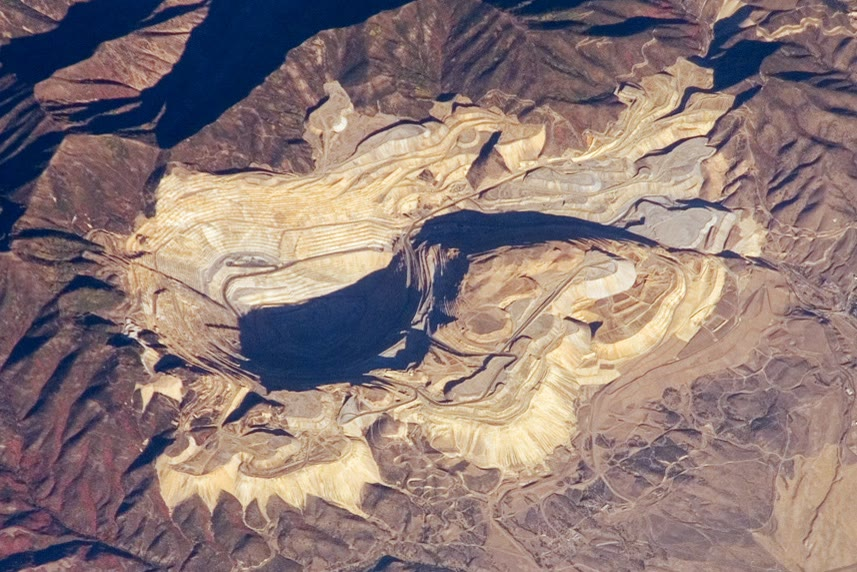
\includegraphics[width=0.5\linewidth]{images/book4/b2-29-bingham-canyon-iss.jpg}
\par\smallskip{\small La corta de Bingham Canyon, Utah, vista desde la Estación Espacial Internacional
(2007): más de \qty{4}{km} de ancho y \qty{1200}{m} de profundidad, excavada en bancos de 16 a \qty{25}{m} de altura
en un \omterm{def:b2:ore-deposits:hydrothermal}{yacimiento de pórfido cuprífero}; las colinas de cima plana que la rodean son escombreras de estéril. Fotografía:
NASA, tripulación de la Expedición 15 (dominio público).}
\end{omfigure}
% ledger: photo:b2-29-bingham

\begin{definition}[Tipos de yacimiento]\label{def:b2:ore-deposits:types}
Un \emph{tipo de yacimiento}\index{tipo de yacimiento} es una clase de yacimientos que comparten un marco
geológico, una roca encajante, una forma, una mineralogía de mena y un proceso de formación, de modo que la descripción de
la clase predice dónde se encuentran sus miembros. Los tipos se agrupan en cuatro familias según el proceso:
magmáticos (el metal lo concentra un \omterm{def:b2:magma-emplacement:magma}{magma} al cristalizar o al separarse en dos líquidos),
hidrotermales (un fluido acuoso caliente), sedimentarios (el transporte y el depósito
de sedimento, o la precipitación a partir del agua en la superficie) y supergénicos (la meteorización
de un yacimiento anterior).
\end{definition}

\section{Yacimientos magmáticos}\label{sec:b2:ore-deposits:magmatic}

\textbf{La cromita de las intrusiones estratificadas.} La cromita, la única fuente comercial de cromo,
se concentra en capas de cromitita masiva, con más del \qty{90}{\percent} de cromita, en las partes inferiores
ultramáficas de las intrusiones estratificadas. Las intrusiones miden de 2 a \qty{180}{km} de diámetro y hasta
\qty{15}{km} de espesor, y las capas van de menos de un centímetro a 5--\qty{8}{m}; juntas
contienen la mayor parte de las reservas mundiales de cromo, y el complejo de Bushveld, visto en el
\cref{ch:b2:magmatic-differentiation}, es la única intrusión que hoy se explota por su cromita. Su origen, una
capa de \omterm{def:b2:magmatic-differentiation:cumulate}{cumulado} llevada al campo de la cromita por la \omterm{def:b2:magmatic-differentiation:open}{mezcla de magmas} o por un cambio de presión o del
estado de oxidación, sigue siendo objeto de debate.
% ledger: usgs10e:chromite

\textbf{Sulfuros de níquel, cobre y EGP.} Un \omterm{def:b2:magma-emplacement:magma}{magma} máfico o ultramáfico, producido por grados elevados de
fusión del manto (del \qty{20}{\percent} al \qty{25}{\percent} o más, con más de un 12 por ciento de MgO en
peso), asciende subsaturado en azufre. Si asimila azufre de la corteza, o se enfría lo
suficiente, se satura y un líquido sulfurado inmiscible se separa en gotas. Los
metales calcófilos pasan a esas gotas: la razón $D$ entre su concentración en el líquido sulfurado
y su concentración en el líquido silicatado, un coeficiente de reparto del mismo tipo que el que hay entre un
mineral y un fundido, vale de $10^2$ a $10^3$ para el cobre y el níquel y de $10^3$ a $10^4$ para los
elementos del grupo del platino (EGP). Cuánto metal reúne una gota depende entonces de cuánto \omterm{def:b2:magma-emplacement:magma}{magma} encuentra.
% ledger: usgs10i:r-factor

\begin{proposition}[Factor R]\label{prop:b2:ore-deposits:r-factor}
Sea una masa unidad de líquido sulfurado que se separa de una masa $R$ de \omterm{def:b2:magma-emplacement:magma}{magma} silicatado, el
\emph{factor R}\index{factor R}, y se equilibra con ella en un sistema cerrado; sea $C_L$ la concentración de un
metal en el \omterm{def:b2:magma-emplacement:magma}{magma} antes de la separación del sulfuro, y $D$ su coeficiente de reparto
sulfuro--silicato. Entonces la concentración del metal en el sulfuro es
\begin{equation}
C_S = C_L\,\frac{D\,(R + 1)}{R + D} .
\label{eq:b2:ore-deposits:r-factor}
\end{equation}
Para $R \gg D$, $C_S \to D\,C_L$; para $R \ll D$, $C_S \approx (R + 1)\,C_L$.
\end{proposition}

\begin{proof}
El sistema de masa $R + 1$ contenía $(R + 1)C_L$ del metal antes de la separación. Después, el silicato
contiene $R\,C_{\mathrm{sil}}$ y el sulfuro $C_S$, con $C_S = D\,C_{\mathrm{sil}}$ en el equilibrio.
La conservación da $(R + 1)C_L = R\,C_S/D + C_S = C_S\,(R + D)/D$, de donde
\eqref{eq:b2:ore-deposits:r-factor}. Si $R \gg D$, $(R + 1)/(R + D) \to 1$; si $R \ll D$,
$D/(R + D) \to 1$.
\end{proof}

Los dos límites explican por qué existen dos clases de mena sulfurada. Cuando $R \ll D$ el sulfuro toma
casi todo el metal del \omterm{def:b2:magma-emplacement:magma}{magma} que encuentra y $C_S$ crece con $R$; cuando $R \gg D$ está
saturado en $D\,C_L$ y más \omterm{def:b2:magma-emplacement:magma}{magma} no añade nada. El níquel y el cobre, con $D$ de unos cientos,
alcanzan su techo con $R$ de unos cientos a unos miles, el intervalo de la mayoría de las menas de níquel y
cobre; el platino y el paladio, con $D$ cercano a $10^4$, siguen ganando hasta $R$ de \num{10000} a
\num{100000}. Las menas ricas en elementos del grupo del platino, como el Merensky Reef del Bushveld y
algunas menas de Norilsk, registran por tanto una pequeña masa de sulfuro lavada por una masa muy grande de
\omterm{def:b2:magma-emplacement:magma}{magma} (ejercicios~\ref{exo:b2:ore-deposits:5} y~\ref{exo:b2:ore-deposits:11}).
% ledger: usgs10i:r-factor

\textbf{Kimberlitas y diamantes.} La mayoría de los diamantes, y casi todos los explotados, se formaron en la base de
una litosfera continental gruesa, en las raíces de los cratones; los \omterm{def:b2:magma-emplacement:magma}{magmas} kimberlíticos, que proceden de profundidades
mayores de 120 a \qty{150}{km} y ascienden hasta a \qty{20}{m.s^{-1}}, los llevan a la
superficie lo bastante deprisa para que sobrevivan. Las kimberlitas hacen erupción preferentemente a través de una litosfera gruesa y antigua,
que es donde busca la exploración de diamantes.
% ledger: grabreck22:kimberlite

\textbf{Pegmatitas.} Las pegmatitas de litio, cesio y tántalo son \omterm{def:b2:magma-emplacement:bodies}{diques} graníticos enriquecidos en estos
elementos raros, producidos en \omterm{def:b2:himalaya-andes:types}{orógenos de colisión}; cristalizan a unos 350 a \qty{550}{\celsius},
una temperatura notablemente baja para un fundido granítico, en días o años, y desarrollan cristales enormes: un
cristal de espodumena medía \qty{14}{m} de largo. Sus minerales de litio, espodumena, petalita y
lepidolita, aportan alrededor de una cuarta parte del litio del mundo.
% ledger: usgs10o:lct

\section{Yacimientos hidrotermales}\label{sec:b2:ore-deposits:hydrothermal}

\begin{definition}[Fluido hidrotermal y tipos de yacimiento hidrotermal]\label{def:b2:ore-deposits:hydrothermal}
Un \emph{fluido hidrotermal}\index{fluido hidrotermal} es un fluido acuoso caliente, liberado por un \omterm{def:b2:magma-emplacement:magma}{magma}
o por reacciones metamórficas, o bien agua de mar, agua meteórica o salmuera de cuenca calentadas, que disuelve,
transporta y deposita elementos al fluir a través de la roca. Los principales \omterm{def:b2:ore-deposits:types}{tipos de yacimiento} hidrotermal
son:
\begin{itemize}
  \item el \emph{yacimiento de pórfido cuprífero}\index{yacimiento de pórfido cuprífero}: un cuerpo grande y de baja \omterm{def:b2:ore-deposits:grade}{ley}
        de vetillas y sulfuros de cobre diseminados en un pequeño stock porfídico y a su alrededor, formado por
        fluidos magmáticos a pocos kilómetros de la superficie por encima de una zona de subducción;
  \item el \emph{yacimiento epitermal}\index{yacimiento epitermal}: filones y diseminaciones de oro y plata
        formados a menos de alrededor de \qty{1.5}{km} de la superficie, a unos 100 a
        \qty{300}{\celsius}, en arcos volcánicos;
  \item el \emph{yacimiento de sulfuros masivos vulcanogénicos}\index{yacimiento de sulfuros masivos vulcanogénicos}
        (VMS, por sus siglas en inglés): una lente de sulfuros masivos formada sobre el fondo marino o justo debajo de él, en una
        surgencia hidrotermal de un entorno volcánico submarino;
  \item el \emph{yacimiento sedimentario exhalativo}\index{yacimiento sedimentario exhalativo} (sedex):
        sulfuros laminados de zinc y plomo en lutitas marinas de una \omterm{def:b2:basins-compared:types}{cuenca de rift}, precipitados sobre el fondo marino o justo
        debajo de él a partir de salmueras de cuenca que ascienden por fallas;
  \item el \emph{yacimiento de tipo Mississippi Valley}\index{yacimiento de tipo Mississippi Valley} (MVT):
        sulfuros de zinc y plomo que reemplazan carbonatos de plataforma, epigenéticos y sin relación con la actividad
        ígnea, depositados por salmueras de cuenca;
  \item el \emph{yacimiento de oro orogénico}\index{yacimiento de oro orogénico}: filones de cuarzo aurífero en
        cinturones metamórficos, a lo largo de grandes fallas, depositados por fluidos de baja salinidad y ricos en CO$_2$, de
        origen metamórfico.
\end{itemize}
\end{definition}
% ledger: usgs10b:form, usgs10q:epithermal, usgs10c:vms, usgs10n:sedex, usgs10a:mvt, drew03:orogenic

\textbf{Transporte y depósito.} La mayoría de los metales viajan en los \omterm{def:b2:ore-deposits:hydrothermal}{fluidos hidrotermales} en forma de complejos:
el zinc, el plomo y el cobre como complejos clorurados, de modo que la salinidad controla su solubilidad, y el oro,
en fluidos reducidos, como complejos de azufre como AuHS(H$_2$S)$_3$. Un fluido deposita su carga cuando la
solubilidad disminuye: cuando se enfría; cuando hierve al bajar su presión, con pérdida de H$_2$S y de CO$_2$ y
cambio de pH; cuando se mezcla con un fluido de composición distinta ---una salmuera que encuentra agua rica
en H$_2$S precipita esfalerita y galena casi al instante---; y cuando reacciona con la roca
encajante, lo que cambia su pH o su estado de oxidación. Cada \omterm{def:b2:ore-deposits:types}{tipo de yacimiento} es una combinación de fluido,
vía de circulación y trampa.
% ledger: usgs10n:sedex, drew03:orogenic

\textbf{Pórfidos cupríferos.} Los yacimientos de pórfido aportan alrededor del \qty{60}{\percent} del cobre del
mundo y contienen alrededor del \qty{65}{\percent} de sus recursos. Se centran en pequeños stocks cilíndricos
o enjambres de \omterm{def:b2:magma-emplacement:bodies}{diques}, las cúpulas de plutones mayores, emplazados a menos de 5--\qty{10}{km} de profundidad en
arcos por encima de zonas de subducción, el marco del \cref{ch:b2:magmatic-series}. Un yacimiento mide de 0.1 a
\qty{1}{km} de diámetro, con una altura similar; la roca alterada puede extenderse \qty{10}{km} o más a su alrededor.
Al cristalizar el \omterm{def:b2:magma-emplacement:magma}{magma}, se separa de él un fluido con un 3 a 5 por ciento de sal en peso; al ascender y
descomprimirse, se divide en una salmuera y un vapor, ambos portadores de metales, y su sobrepresión
fractura la roca. Los filones de cuarzo precipitan a unos 700 a \qty{500}{\celsius}, y la
reacción del fluido con la roca zona la alteración, como en el corte de abajo. Como se
forman a poca profundidad en márgenes activos, donde la erosión es rápida, más del \qty{90}{\percent} de los
yacimientos de pórfido conocidos son cenozoicos o mesozoicos.
% ledger: usgs10b:share, usgs10b:form, usgs10b:fluids, usgs10b:alteration

\begin{omfigure}
\centering
\begin{tikzpicture}[x=1.15cm, y=1.15cm, font=\small]
\begin{scope}
\clip (-2.9,-3.6) rectangle (2.9,0);
% propylitic halo
\fill[omLithBasalt!45] (0,-1.25) ellipse (2.45 and 1.55);
% sodic-calcic deep flanks
\fill[omExo!25] (-1.75,-2.55) ellipse (0.45 and 0.38);
\fill[omExo!25] (1.75,-2.55) ellipse (0.45 and 0.38);
% sericitic shell
\fill[yellow!35] (0,-1.05) ellipse (1.15 and 1.15);
% potassic core
\fill[omProp!40] (0,-1.45) ellipse (0.68 and 0.85);
% ore shell
\draw[omThm, line width=1.1pt, densely dashed] (0,-1.3) ellipse (0.92 and 0.98);
% advanced argillic lithocap
\fill[omDef!30] (-1.05,0) .. controls (-0.6,-0.5) and (0.6,-0.5) .. (1.05,0) -- cycle;
\draw[omDef!70] (-1.05,0) .. controls (-0.6,-0.5) and (0.6,-0.5) .. (1.05,0);
\end{scope}
% pluton and stock
\fill[omLithGranite] (-2.6,-3.6) .. controls (-2.2,-2.9) and (-0.9,-2.6) .. (-0.3,-2.6)
  -- (-0.3,-1.25) arc[start angle=180, end angle=0, radius=0.3] -- (0.3,-2.6)
  .. controls (0.9,-2.6) and (2.2,-2.9) .. (2.6,-3.6) -- cycle;
\draw[black!60] (-2.6,-3.6) .. controls (-2.2,-2.9) and (-0.9,-2.6) .. (-0.3,-2.6)
  -- (-0.3,-1.25) arc[start angle=180, end angle=0, radius=0.3] -- (0.3,-2.6)
  .. controls (0.9,-2.6) and (2.2,-2.9) .. (2.6,-3.6);
% epithermal veins
\foreach \x in {1.45,1.65,1.85} \draw[omDef, line width=1pt] (\x,-0.02) -- (\x+0.12,-0.7);
% palaeosurface
\draw[black, line width=0.8pt] (-2.9,0) -- (2.9,0);
\node[anchor=south west, font=\scriptsize] at (-2.9,0) {paleosuperficie};
% labels
\draw[black!50] (0.6,-0.15) -- (1.2,0.25) -- (3.0,0.25) node[anchor=west, text=black] {argílica avanzada};
\draw[black!50] (1.95,-0.3) -- (3.0,-0.3) node[anchor=west, text=black] {filones epitermales};
\draw[black!50] (1.05,-0.8) -- (3.0,-0.8) node[anchor=west, text=black] {sericítica};
\draw[black!50] (0.85,-1.25) -- (3.0,-1.25) node[anchor=west, text=omThm] {envolvente de mena de cobre};
\draw[black!50] (0.45,-1.7) -- (3.0,-1.7) node[anchor=west, text=black] {potásica};
\draw[black!50] (1.05,-2.15) -- (3.0,-2.15) node[anchor=west, text=black] {propilítica};
\draw[black!50] (2.1,-2.6) -- (3.0,-2.6) node[anchor=west, text=black] {sódico--cálcica};
\draw[black!50] (1.5,-3.15) -- (3.0,-3.15) node[anchor=west, text=black] {plutón y stock porfídico};
\end{tikzpicture}
\par\smallskip{\small Un sistema de pórfido cuprífero en corte (un dibujo, sin escala): la zona potásica
en el núcleo, profunda y caliente; la zona sericítica hacia arriba y hacia fuera, donde la pirita es
abundante; la envolvente de mena de cobre entre ambas; el halo propilítico a profundidades someras o moderadas
alrededor; la alteración sódico--cálcica en los flancos profundos; un casquete argílico avanzado y, en algunos
sistemas, filones epitermales cerca de la superficie.}
\end{omfigure}
% ledger: usgs10b:alteration

\textbf{Oro epitermal.} Por encima de algunos sistemas porfídicos, y en los arcos volcánicos en general, el mismo
tipo de fluidos alcanza los \qty{1.5}{km} superiores de la corteza a unos 100 a \qty{300}{\celsius},
donde hierven y se mezclan con el agua subterránea; depositan oro y plata en filones de cuarzo, con una
alteración que registra fluidos casi neutros (adularia, illita) o muy ácidos (caolinita,
dickita, pirofilita).
% ledger: usgs10q:epithermal, usgs10q:alteration

\textbf{Sulfuros masivos en el fondo marino.} El agua de mar que desciende hacia la corteza caliente de una dorsal o de
un arco vuelve a salir por surgencias en forma de fumarolas negras a unos \qty{350}{\celsius}, observadas por primera vez en la dorsal del
Pacífico Oriental en 1979. Donde el campo de surgencias perdura, sus sulfuros edifican un montículo; la mena tiene más del
\qty{40}{\percent} de sulfuros, sobre un stockwork de filones que marca el conducto de alimentación. Los metales se zonan
según la temperatura, el hierro y el cobre en la base caliente, el zinc, el hierro, el plomo y el bario en la cima y los
márgenes, más fríos, como en el montículo dibujado en la sección siguiente. Los \omterm{def:b2:ore-deposits:hydrothermal}{yacimientos de sulfuros masivos vulcanogénicos}
van desde bolsadas de menos de una tonelada hasta las \qty{1.5}{Gt} de Río Tinto, en España, y en
edad desde \qty{3.55}{\Ga} hasta yacimientos que se forman hoy.
% ledger: usgs10c:vms

\textbf{Salmueras de cuenca: sedex y MVT.} Las salmueras de cuenca, con un 10 a un \qty{30}{\percent} de sales disueltas y
calentadas a 100--\qty{200}{\celsius} por el enterramiento, transportan zinc y plomo como complejos clorurados y forman los
dos tipos alojados en sedimentos. Los yacimientos sedex se forman donde la salmuera sale a una cuenca restringida y reductora
a lo largo de una falla de rift y encuentra sulfuro de hidrógeno, lo que produce fangos sulfurados laminados; contienen más
de la mitad de las reservas mundiales de zinc y plomo. Los yacimientos MVT se forman donde la salmuera, expulsada de una
cuenca, alcanza una plataforma carbonatada en su margen y la reemplaza a temperaturas de 75 a unos
\qty{200}{\celsius}; contienen el \qty{38}{\percent} del plomo y el zinc de los yacimientos alojados en sedimentos,
con unas diez veces más zinc que plomo.
% ledger: usgs10n:sedex, usgs10a:mvt

\textbf{Oro orogénico.} En los cinturones metamórficos, las reacciones de desvolatilización liberan un fluido casi neutro,
de baja salinidad y rico en CO$_2$; canalizado a lo largo de grandes fallas, deposita filones de cuarzo aurífero
a unos \qty{350}{\celsius} y de 4 a \qty{12}{km} de profundidad. Los filones son continuos en
grandes alturas: \qty{3.2}{km} en Kolar, en la India.
% ledger: drew03:orogenic

\section{Yacimientos sedimentarios y supergénicos}\label{sec:b2:ore-deposits:sedimentary}

\begin{definition}[Placer]\label{def:b2:ore-deposits:placer}
Un \emph{placer}\index{placer} es un yacimiento sedimentario de minerales densos y resistentes concentrados por
el agua o el viento en movimiento porque, a igual tamaño, sedimentan más deprisa y son arrastrados con menos facilidad
que los granos de cuarzo que los rodean.
\end{definition}

Los minerales de densidad superior a unos 2.85 se llaman pesados, frente a 2.65 para el cuarzo: la ilmenita y el circón
rondan 4.7, la magnetita 5.2, el oro de 15 a 19.3. Según la ley de Stokes, la velocidad de sedimentación de un grano crece con
su exceso de densidad $\rho_s - \rho_w$, once veces mayor para el oro que para el cuarzo, de modo que el oro de un
tamaño dado se encuentra con cuarzo tres veces mayor (\cref{exo:b2:ore-deposits:3}); el oro
suele quedarse en las gravas fluviales sobre el sustrato rocoso, mientras que la ilmenita, el rutilo y el circón llegan a las playas y
las dunas. Las \omterm{def:b2:ore-deposits:grade}{leyes} de las arenas de minerales pesados son el tanto por ciento en peso de minerales pesados.
% ledger: usgs10l:heavy, usgs:gold-placer

Los sedimentos químicos también son menas. Las formaciones de hierro bandeado del \cref{ch:b2:precambrian-earth},
precipitadas a medida que se oxidaba el hierro disuelto de los océanos, son una mena común de hierro; las evaporitas
aportan halita y las sales de potasio; las lateritas, el residuo de una meteorización tropical profunda,
concentran el aluminio en forma de bauxita. La meteorización también enriquece yacimientos anteriores.
% ledger: earle:bif, usgs:bauxite

\begin{definition}[Enriquecimiento supergénico, gossan]\label{def:b2:ore-deposits:supergene}
El \emph{enriquecimiento supergénico}\index{enriquecimiento supergénico} es la concentración de un metal por
el agua subterránea descendente: por encima del nivel freático, el agua oxigenada y ácida disuelve el metal de los
sulfuros de un cuerpo mineralizado, y por debajo de él, en condiciones reductoras, lo vuelve a depositar, sobre todo
reemplazando los sulfuros primarios. Un \emph{gossan}\index{gossan} (o sombrero de hierro) es la roca porosa, rica en óxidos de hierro,
que queda en la superficie sobre un cuerpo sulfurado meteorizado, con sus sulfuros reemplazados por goethita, hematites y
jarosita.
\end{definition}

En los yacimientos de pórfido, la zona lixiviada por encima del nivel freático alcanza hasta varios cientos de metros
de espesor; por debajo, las zonas de sulfuros enriquecidos en calcosina, de decenas a varios cientos de metros de espesor, llegan a
más de \qty{1.5}{Gt} con un 0.4 a un \qty{1.7}{\percent} de cobre, siempre más ricas que la mena primaria,
hipogénica, que hay debajo. Los óxidos de hierro de un \omterm{def:b2:ore-deposits:supergene}{gossan} y de una zona lixiviada conservan las texturas de los
sulfuros que reemplazaron y guían la búsqueda en profundidad; los \omterm{def:b2:ore-deposits:supergene}{gossans} y sus manchas de hierro revelaron muchos
yacimientos de sulfuros masivos a los primeros mineros.
% ledger: usgs10b:supergene, usgs10c:vms

\begin{omfigure}
\centering
\begin{minipage}[b]{0.46\linewidth}\centering
\begin{tikzpicture}[x=1cm, y=1cm, font=\scriptsize]
\fill[omHist!55] (0,4.0) rectangle (1.8,5.2);
\fill[omMeth!30] (0,3.0) rectangle (1.8,4.0);
\fill[black!55] (0,1.8) rectangle (1.8,3.0);
\fill[black!18] (0,0) rectangle (1.8,1.8);
\draw (0,0) rectangle (1.8,5.2);
\draw[omDef, line width=1pt, densely dashed] (-0.25,3.0) -- (2.05,3.0);
\foreach \x in {0.45,0.9,1.35} \draw[omDef, -{Stealth[length=4pt]}] (\x,5.0) -- (\x,3.2);
\node[anchor=west, align=left] at (2.0,4.6) {gossan y zona\\lixiviada (óxidos de Fe)};
\node[anchor=west, align=left] at (2.0,3.5) {zona de óxidos\\(malaquita)};
\node[anchor=east, text=omDef, align=right] at (-0.25,3.0) {nivel\\freático};
\node[anchor=west, align=left] at (2.0,2.4) {zona de enriquecimiento\\(calcosina)};
\node[anchor=west, align=left] at (2.0,0.9) {mena primaria\\(calcopirita\\+ pirita)};
\node[anchor=south, font=\scriptsize, text=omDef] at (0.9,5.25) {agua ácida, Cu$^{2+}$};
\end{tikzpicture}
\end{minipage}\hfill
\begin{minipage}[b]{0.52\linewidth}\centering
\begin{tikzpicture}[x=1cm, y=1cm, font=\scriptsize]
\fill[omSea] (-2.6,1.4) rectangle (2.6,3.2);
\fill[omLithBasalt!60] (-2.6,-1.6) rectangle (2.6,1.4);
% stockwork cone
\fill[omProp!25] (-0.5,-1.6) -- (0.5,-1.6) -- (1.1,0.9) -- (-1.1,0.9) -- cycle;
\foreach \x/\y in {-0.3/-1.2,0.1/-1.0,-0.6/-0.4,0.4/-0.3,-0.1/0.1,0.6/0.4,-0.7/0.5}
  \draw[omProp!80!black] (\x,\y) -- ++(0.35,0.25);
% mound: upper rim and core
\fill[yellow!45] (-1.8,1.4) .. controls (-1.2,2.35) and (1.2,2.35) .. (1.8,1.4) -- cycle;
\fill[omThm!45] (-1.1,1.4) .. controls (-0.7,2.0) and (0.7,2.0) .. (1.1,1.4) -- cycle;
\draw (-1.8,1.4) .. controls (-1.2,2.35) and (1.2,2.35) .. (1.8,1.4);
% chimney and plume
\fill[black!70] (-0.08,2.1) rectangle (0.08,2.55);
\fill[black!45] (0,2.6) circle (0.12) (0.1,2.8) circle (0.16) (0.25,3.0) circle (0.2);
\draw[omDef, -{Stealth[length=4pt]}] (-2.3,2.9) -- (-2.3,0.2) -- (-1.2,-0.9);
\draw[omThm, -{Stealth[length=4pt]}] (0,-1.5) -- (0,1.2);
\node[anchor=west, text=omDef] at (-2.55,3.05) {agua de mar};
\node[anchor=west] at (0.45,2.85) {fumarola negra, \qty{350}{\celsius}};
\draw[black!50] (1.45,1.75) -- (2.0,2.15) node[anchor=west, text=black] {Zn, Fe, Pb, Ba};
\draw[black!50] (0.6,1.6) -- (2.0,1.15) node[anchor=west, text=black] {Fe, Cu};
\node[anchor=west, align=left] at (0.95,-0.4) {stockwork\\(conducto)};
\node[anchor=north, text=omThm] at (0,-1.6) {fluido caliente};
\end{tikzpicture}
\end{minipage}
\par\smallskip{\small Izquierda: un perfil supergénico sobre un cuerpo de sulfuros de cobre (un dibujo, sin
escala): el agua ácida lixivia el cobre por encima del nivel freático y lo vuelve a depositar como calcosina por debajo,
dejando un \omterm{def:b2:ore-deposits:supergene}{gossan} en la superficie. Derecha: un montículo de sulfuros masivos vulcanogénicos en corte (un
dibujo): el agua de mar calentada en la corteza asciende por un stockwork y sale como fumarola negra; el
montículo está zonado desde el hierro y el cobre en la base caliente hasta el zinc, el hierro, el plomo y el bario en la cima y los
márgenes.}
\end{omfigure}
% ledger: usgs10b:supergene, usgs10c:vms

\begin{omfigure}
\centering
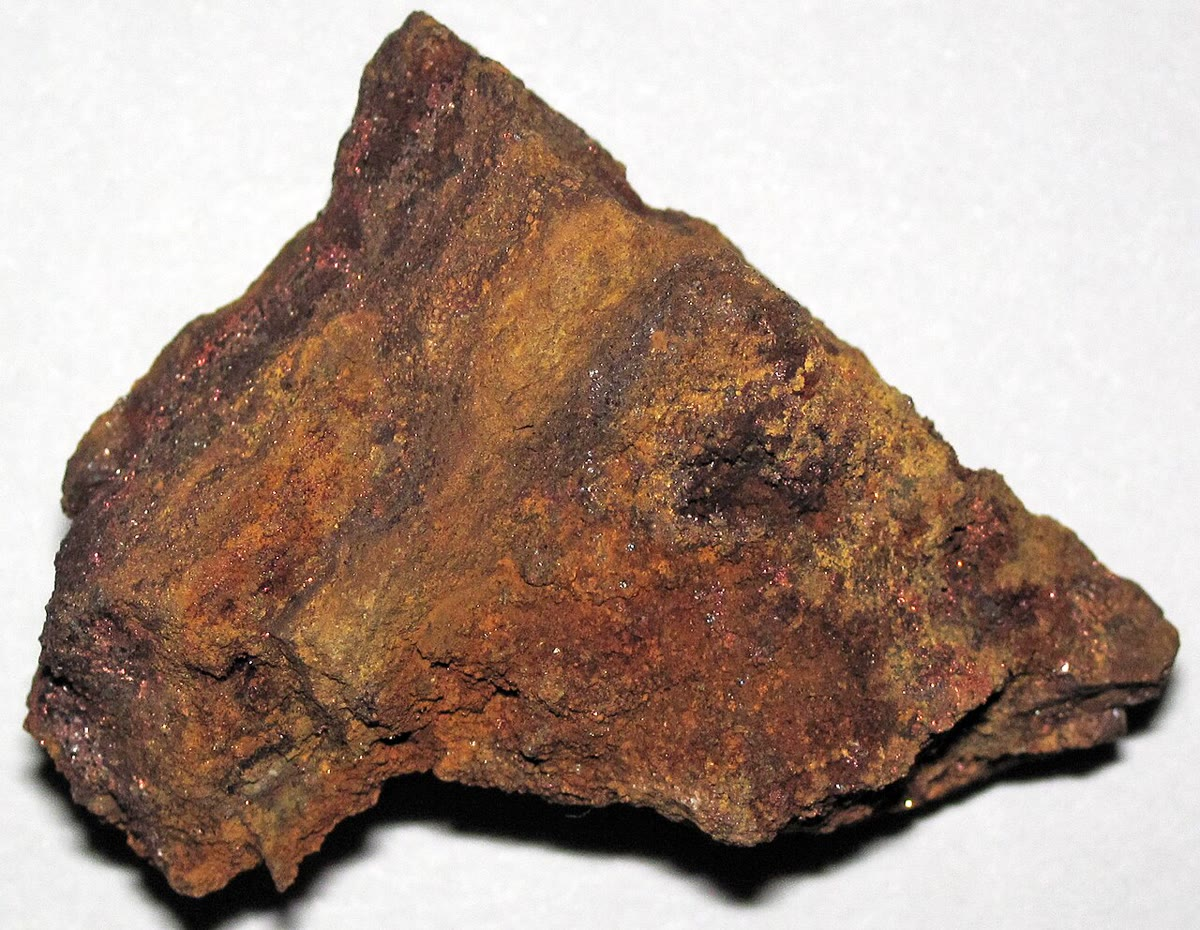
\includegraphics[width=0.4\linewidth]{images/book4/b2-29-flambeau-gossan.jpg}
\par\smallskip{\small \omterm{def:b2:ore-deposits:supergene}{Gossan} del yacimiento de sulfuros masivos de Flambeau, Wisconsin: una roca porosa de
oxihidróxidos de hierro dejada por la meteorización de pirita, calcopirita, calcosina y bornita en un
arco volcánico paleoproterozoico; las pequeñas motas anaranjadas son cobre nativo. Fotografía: James St.
John (CC BY 2.0).}
\end{omfigure}
% ledger: photo:b2-29-gossan

\section{Ley y tonelaje}\label{sec:b2:ore-deposits:grade-tonnage}

Una compilación mundial recoge 422 \omterm{def:b2:ore-deposits:hydrothermal}{yacimientos de pórfido cuprífero} con su \omterm{def:b2:ore-deposits:grade}{tonelaje}, para la \omterm{def:b2:ore-deposits:grade}{ley de corte} más baja
disponible, y su \omterm{def:b2:ore-deposits:grade}{ley} media de cobre. Una décima parte supera las \qty{1500}{Mt} y otra décima parte contiene menos
de \qty{33}{Mt}, con una mediana de \qty{240}{Mt}; las \omterm{def:b2:ore-deposits:grade}{leyes} van del \qty{0.24}{\percent} al
\qty{0.75}{\percent} entre los mismos deciles, con una mediana del \qty{0.44}{\percent}. Entre los
deciles, el \omterm{def:b2:ore-deposits:grade}{tonelaje} se extiende sobre un factor de 45 y la \omterm{def:b2:ore-deposits:grade}{ley} sobre un factor de 3. En ejes logarítmicos, ambos histogramas se acercan a curvas normales, como muestra la figura siguiente:
los logaritmos del \omterm{def:b2:ore-deposits:grade}{tonelaje} tienen una media de 2.373 y una desviación típica de 0.654, los de la \omterm{def:b2:ore-deposits:grade}{ley}
$-0.364$ y 0.199 (logaritmos en base 10, \omterm{def:b2:ore-deposits:grade}{tonelaje} en megatoneladas, \omterm{def:b2:ore-deposits:grade}{ley} en tanto por ciento). El ajuste es
imperfecto: las \omterm{def:b2:ore-deposits:grade}{leyes} son más apuntadas que una ley lognormal, y unos pocos yacimientos de \omterm{def:b2:ore-deposits:grade}{ley} muy baja hacen
que se aparten de ella en un contraste formal. Además, ambos son casi independientes, con una correlación de
0.1 entre sus logaritmos.
% ledger: usgs08:table1, usgs08:independence, data:b4-porphyry-cu

\begin{omfigure}
\centering
\begin{minipage}[b]{0.49\linewidth}\centering
\begin{tikzpicture}
\begin{axis}[omrecord, width=0.96\linewidth, height=4.5cm, xmin=0.5, xmax=5.0, ymin=0, ymax=80,
  xlabel={tonelaje (Mt)}, ylabel={número de yacimientos},
  xtick={1,2,3,4,5}, xticklabels={10,100,1000,$10^4$,$10^5$},
  tick label style={font=\scriptsize}, label style={font=\small}]
% computed in figdata/bachelor-2/ores.py part hist_t; ledger: data:b4-porphyry-cu
\addplot[ybar, bar width=0.22, fill=omDef!35, draw=omDef!70] table[x=log10_t, y=count] {figdata/out/bachelor-2-ores-hist_t.dat};
\addplot[omThm, line width=1pt, smooth] table[x=log10_t, y=fit] {figdata/out/bachelor-2-ores-hist_t.dat};
\end{axis}
\end{tikzpicture}
\end{minipage}\hfill
\begin{minipage}[b]{0.49\linewidth}\centering
\begin{tikzpicture}
\begin{axis}[omrecord, width=0.96\linewidth, height=4.5cm, xmin=-1.2, xmax=0.6, ymin=0, ymax=120,
  xlabel={ley de cobre (\%)}, ylabel={número de yacimientos},
  xtick={-1,-0.69897,-0.30103,0,0.30103}, xticklabels={0.1,0.2,0.5,1,2},
  tick label style={font=\scriptsize}, label style={font=\small}]
% computed in figdata/bachelor-2/ores.py part hist_g; ledger: data:b4-porphyry-cu
\addplot[ybar, bar width=0.088, fill=omDef!35, draw=omDef!70] table[x=log10_g, y=count] {figdata/out/bachelor-2-ores-hist_g.dat};
\addplot[omThm, line width=1pt, smooth] table[x=log10_g, y=fit] {figdata/out/bachelor-2-ores-hist_g.dat};
\end{axis}
\end{tikzpicture}
\end{minipage}
\par\smallskip{\small El \omterm{def:b2:ore-deposits:grade}{tonelaje} (izquierda) y la \omterm{def:b2:ore-deposits:grade}{ley} de cobre (derecha) de los 422 \omterm{def:b2:ore-deposits:hydrothermal}{yacimientos de pórfido cuprífero}
de la compilación mundial, en ejes logarítmicos, con las curvas normales de la misma media
y desviación típica en rojo. Datos: Singer, Berger y Moring (2008), USGS.}
\end{omfigure}

\begin{proposition}[Producto de variables lognormales]\label{prop:b2:ore-deposits:product}
Si $\log_{10} T$ y $\log_{10} g$ son conjuntamente normales, con medias $\mu_T$ y $\mu_g$, desviaciones
típicas $\sigma_T$ y $\sigma_g$ y correlación $\rho$, entonces el metal contenido $M = Tg/100$
($g$ en tanto por ciento) es lognormal: $\log_{10} M$ es normal con
\begin{equation}
\mu_M = \mu_T + \mu_g - 2 , \qquad
\sigma_M^2 = \sigma_T^2 + \sigma_g^2 + 2\rho\,\sigma_T\sigma_g .
\label{eq:b2:ore-deposits:product}
\end{equation}
\end{proposition}

\begin{proof}
$\log_{10} M = \log_{10} T + \log_{10} g - 2$. Una combinación lineal de variables conjuntamente normales es
normal (se admite de los libros de matemáticas); su media es la suma de las medias y su varianza
$\operatorname{var}(X + Y) = \operatorname{var} X + \operatorname{var} Y + 2\operatorname{cov}(X, Y)$,
con $\operatorname{cov}(X, Y) = \rho\,\sigma_T\sigma_g$.
\end{proof}

Para los yacimientos de pórfido, $\sigma_M = \sqrt{0.654^2 + 0.199^2 + 2 \times 0.1 \times 0.654 \times
0.199} = 0.702$ y $\mu_M = 0.009$: el yacimiento mediano contiene alrededor de \qty{1}{Mt} de cobre, y el
metal contenido se dispersa todavía más que el \omterm{def:b2:ore-deposits:grade}{tonelaje}. Una ley lognormal con una dispersión tan grande
pone la mayor parte del metal en unos pocos yacimientos: la décima parte mayor contiene alrededor del \qty{63}{\percent} del
cobre según la ley, el \qty{64}{\percent} en los datos (\cref{exo:b2:ore-deposits:12}). La
figura siguiente representa cada yacimiento por su \omterm{def:b2:ore-deposits:grade}{tonelaje} y su \omterm{def:b2:ore-deposits:grade}{ley}, con líneas de igual cobre contenido;
Bingham, con \qty{28.5}{Mt}, queda entre las líneas de 10 y de \qty{100}{Mt}.
% ledger: data:b4-porphyry-cu
% values: sd_log10_m 0.702233, mean 0.00857; median M 1.02 Mt; top 10 % share 0.631 (fit) 0.643 (data)

\begin{definition}[Curva ley--tonelaje]\label{def:b2:ore-deposits:gt}
La \emph{curva ley--tonelaje}\index{curva ley--tonelaje} de un yacimiento da, en función de
la \omterm{def:b2:ore-deposits:grade}{ley de corte} $c$, el \omterm{def:b2:ore-deposits:grade}{tonelaje} $T(c)$ de los bloques con \omterm{def:b2:ore-deposits:grade}{ley} superior a $c$ y su \omterm{def:b2:ore-deposits:grade}{ley} media
$\bar g(c)$.
\end{definition}

\begin{proposition}[Curva ley--tonelaje de un yacimiento lognormal]\label{prop:b2:ore-deposits:gt}
Si las \omterm{def:b2:ore-deposits:grade}{leyes} de los bloques de un yacimiento de \omterm{def:b2:ore-deposits:grade}{tonelaje} total $T_0$ son lognormales, con $\ln g$ normal
de media $\mu$ (la \omterm{def:b2:ore-deposits:grade}{ley} mediana es $e^{\mu}$) y desviación típica $s$, entonces, con $z = (\mu -
\ln c)/s$,
\begin{equation}
T(c) = T_0\,\Phi(z), \qquad
\bar g(c) = e^{\mu + s^2/2}\,\frac{\Phi(z + s)}{\Phi(z)} ,
\label{eq:b2:ore-deposits:gt}
\end{equation}
y el metal por encima de la \omterm{def:b2:ore-deposits:grade}{ley de corte} es $M(c) = T_0\,e^{\mu + s^2/2}\,\Phi(z + s)$, una fracción $\Phi(z +
s)$ del total.
\end{proposition}

\begin{proof}
Escríbase $\ln g = \mu + s u$, con $u$ normal tipificada. Un bloque está por encima de la \omterm{def:b2:ore-deposits:grade}{ley de corte} cuando $u > (\ln c -
\mu)/s = -z$, lo que tiene probabilidad $1 - \Phi(-z) = \Phi(z)$; de ahí $T(c)$. El metal por encima de la
\omterm{def:b2:ore-deposits:grade}{ley de corte} por unidad de \omterm{def:b2:ore-deposits:grade}{tonelaje} total es $\int_{-z}^{\infty} e^{\mu + s u}\,\varphi(u)\,\mathrm{d}u$,
con $\varphi$ la densidad normal tipificada. Completando el cuadrado, $e^{su}\varphi(u) =
e^{s^2/2}\varphi(u - s)$, así que la integral vale $e^{\mu + s^2/2}\,[1 - \Phi(-z - s)] = e^{\mu +
s^2/2}\,\Phi(z + s)$. Dividir por $\Phi(z)$ da la \omterm{def:b2:ore-deposits:grade}{ley} media.
\end{proof}

Cuando $c \to 0$ se conserva todo el yacimiento, con la \omterm{def:b2:ore-deposits:grade}{ley} media $e^{\mu + s^2/2}$, que es superior a la
mediana. Subir la \omterm{def:b2:ore-deposits:grade}{ley de corte} elimina \omterm{def:b2:ore-deposits:grade}{tonelaje} más deprisa que metal, porque los bloques eliminados son los
más pobres: en el yacimiento ilustrativo de la figura, subir la \omterm{def:b2:ore-deposits:grade}{ley de corte} del 0.2 al
\qty{0.5}{\percent} conserva el \qty{41}{\percent} del \omterm{def:b2:ore-deposits:grade}{tonelaje} pero el \qty{61}{\percent} del cobre.
% values: demo T 876.0/355.0 Mt, M 4.599/2.826 Mt (figdata ores.py gtcurve)

\begin{omfigure}
\centering
\begin{minipage}[b]{0.49\linewidth}\centering
\begin{tikzpicture}
\begin{axis}[omrecord, width=0.96\linewidth, height=5.0cm, xmode=log, ymode=log,
  xmin=2, xmax=50000, ymin=0.05, ymax=2.8, xlabel={tonelaje (Mt)}, ylabel={ley de cobre (\%)},
  ytick={0.1,0.2,0.5,1,2}, yticklabels={0.1,0.2,0.5,1,2},
  tick label style={font=\scriptsize}, label style={font=\small}]
% computed in figdata/bachelor-2/ores.py parts scatter and iso; ledger: data:b4-porphyry-cu
\addplot[black!45, line width=0.6pt, unbounded coords=jump] table[x=tonnage_mt, y=g01] {figdata/out/bachelor-2-ores-iso.dat};
\addplot[black!45, line width=0.6pt, unbounded coords=jump] table[x=tonnage_mt, y=g1] {figdata/out/bachelor-2-ores-iso.dat};
\addplot[black!45, line width=0.6pt, unbounded coords=jump] table[x=tonnage_mt, y=g10] {figdata/out/bachelor-2-ores-iso.dat};
\addplot[black!45, line width=0.6pt, unbounded coords=jump] table[x=tonnage_mt, y=g100] {figdata/out/bachelor-2-ores-iso.dat};
\addplot[omDef, only marks, mark=*, mark size=0.8pt, opacity=0.7] table[x=tonnage_mt, y=cu_pct] {figdata/out/bachelor-2-ores-scatter.dat};
\addplot[omThm, only marks, mark=square*, mark size=2pt] coordinates {(3230,0.882)};
\node[font=\tiny, text=black!70, fill=white, inner sep=1pt] at (axis cs:4.55,2.2) {0.1};
\node[font=\tiny, text=black!70, fill=white, inner sep=1pt] at (axis cs:45.5,2.2) {1};
\node[font=\tiny, text=black!70, fill=white, inner sep=1pt] at (axis cs:455,2.2) {10};
\node[font=\tiny, text=black!70, fill=white, inner sep=1pt] at (axis cs:4545,2.2) {100 Mt};
\node[font=\scriptsize, text=omThm, anchor=south, fill=white, inner sep=1pt] at (axis cs:3230,1.0) {Bingham};
\end{axis}
\end{tikzpicture}
\end{minipage}\hfill
\begin{minipage}[b]{0.49\linewidth}\centering
\begin{tikzpicture}
\begin{axis}[omrecord, width=0.80\linewidth, height=5.0cm, xmin=0, xmax=1.2, ymin=0, ymax=1000,
  xlabel={ley de corte (\%)}, ylabel={tonelaje sobre el corte (Mt)}, axis y line*=left,
  ylabel style={text=omDef}, tick label style={font=\scriptsize}, label style={font=\small}]
% computed in figdata/bachelor-2/ores.py part gtcurve (illustrative deposit)
\addplot[omDef, line width=1.1pt] table[x=cutoff_pct, y=tonnage_mt] {figdata/out/bachelor-2-ores-gtcurve.dat};
\end{axis}
\begin{axis}[width=0.80\linewidth, height=5.0cm, xmin=0, xmax=1.2, ymin=0, ymax=1.6,
  axis y line*=right, axis x line=none, ylabel={ley media sobre el corte (\%)},
  ylabel style={text=omThm}, tick label style={font=\scriptsize}, label style={font=\small}]
\addplot[omThm, line width=1.1pt, densely dashed] table[x=cutoff_pct, y=grade_pct] {figdata/out/bachelor-2-ores-gtcurve.dat};
\end{axis}
\end{tikzpicture}
\end{minipage}
\par\smallskip{\small Izquierda: \omterm{def:b2:ore-deposits:grade}{tonelaje} y \omterm{def:b2:ore-deposits:grade}{ley} de cobre de los 422 \omterm{def:b2:ore-deposits:hydrothermal}{yacimientos de pórfido cuprífero}, con
líneas de igual cobre contenido (de 0.1 a \qty{100}{Mt}); el cuadrado rojo es Bingham Canyon. Datos:
Singer, Berger y Moring (2008), USGS. Derecha: la \omterm{def:b2:ore-deposits:gt}{curva ley--tonelaje} de un yacimiento ilustrativo
de \qty{1000}{Mt}, \omterm{def:b2:ore-deposits:grade}{ley} mediana del \qty{0.40}{\percent}, $s = 0.60$: \omterm{def:b2:ore-deposits:grade}{tonelaje} por encima de la \omterm{def:b2:ore-deposits:grade}{ley de corte} (azul)
y su \omterm{def:b2:ore-deposits:grade}{ley} media (rojo, discontinua), según \eqref{eq:b2:ore-deposits:gt}.}
\end{omfigure}

\section{Exploración}\label{sec:b2:ore-deposits:exploration}

Los yacimientos se encuentran por las huellas que dejan más allá de su mena. El halo de alteración de un sistema
porfídico tiene kilómetros de ancho y, donde la roca aflora, sus minerales pueden cartografiarse desde aviones
y satélites por sus espectros infrarrojos; sus metales se dispersan en los suelos, los sedimentos fluviales, las aguas y las plantas de su
entorno; y sus sulfuros y rocas alteradas cambian las propiedades físicas que mide la geofísica.
% ledger: usgs10b:form, usgs10b:exploration, usgs10b:remote

\begin{definition}[Anomalía geoquímica]\label{def:b2:ore-deposits:exploration}
Una \emph{anomalía geoquímica}\index{anomalía geoquímica} es una concentración de un elemento, o de un
grupo de elementos, en un medio muestreado ---roca, suelo, sedimento fluvial, agua, plantas--- que
se aparta de su fondo en la región, el intervalo de concentraciones que se encuentra donde no hay
mineralización.
\end{definition}

Como las \omterm{def:b2:ore-deposits:grade}{leyes}, las concentraciones se extienden sobre varios órdenes de magnitud, de modo que una anomalía suele juzgarse sobre
los logaritmos; un umbral sencillo, usado en el \cref{exo:b2:ore-deposits:9}, es la media de
los logaritmos del fondo más dos veces su desviación típica. Una muestra de sedimento fluvial
mezcla el sedimento de toda su cuenca, de modo que una anomalía se atenúa aguas abajo a medida que se le une sedimento limpio,
y el gradiente de las concentraciones apunta aguas arriba, por la red de drenaje, hacia la fuente. En suelos sobre
pegmatitas enterradas se han seguido anomalías de litio, rubidio, cesio, tántalo y estaño por encima de
cuerpos que no afloran.
% ledger: usgs10b:exploration, usgs10o:lct

Los métodos geofísicos se eligen por el contraste que ofrece un \omterm{def:b2:ore-deposits:types}{tipo de yacimiento}. Los sulfuros diseminados hacen que una
roca se comporte como un condensador: el método de polarización inducida, que mide esta cargabilidad, se
desarrolló para los pórfidos cupríferos y responde sobre todo a la zona sericítica rica en pirita, ya que el núcleo
potásico es más pobre en sulfuros. Las prospecciones magnéticas y gravimétricas cartografían los plutones con los que se relacionan
los yacimientos. Ningún método ve la mena
directamente, y toda interpretación es no única hasta que un sondeo la pone a prueba.
% ledger: usgs10b:exploration

\begin{method}[De los análisis a una estimación de recursos]\label{met:b2:ore-deposits:resource}
Los datos son sondeos dispuestos en una malla sobre el yacimiento, con su testigo descrito y analizado por tramos
de longitud conocida.
\begin{enumerate}
  \item \textbf{Compósitos.} Promédiense los análisis sobre longitudes iguales, ponderando cada análisis por su
        longitud, para que cada compósito represente el mismo volumen.
  \item \textbf{Modelo.} Divídase el yacimiento en bloques y estímese la \omterm{def:b2:ore-deposits:grade}{ley} de cada uno a partir de los
        compósitos cercanos, ponderándolos según la distancia y la correlación espacial de las \omterm{def:b2:ore-deposits:grade}{leyes}
        (el método geoestadístico del krigeado, que se admite).
  \item \textbf{Informe.} Aplíquese una \omterm{def:b2:ore-deposits:grade}{ley de corte}: \omterm{def:b2:ore-deposits:grade}{tonelaje} y \omterm{def:b2:ore-deposits:grade}{ley} media de los bloques que la superan, con la
        densidad de la roca, en cada nivel de confianza que permita el espaciado de los sondeos.
\end{enumerate}
\end{method}

\begin{inthefield}[Descripción de testigos de sondeo]
\centering
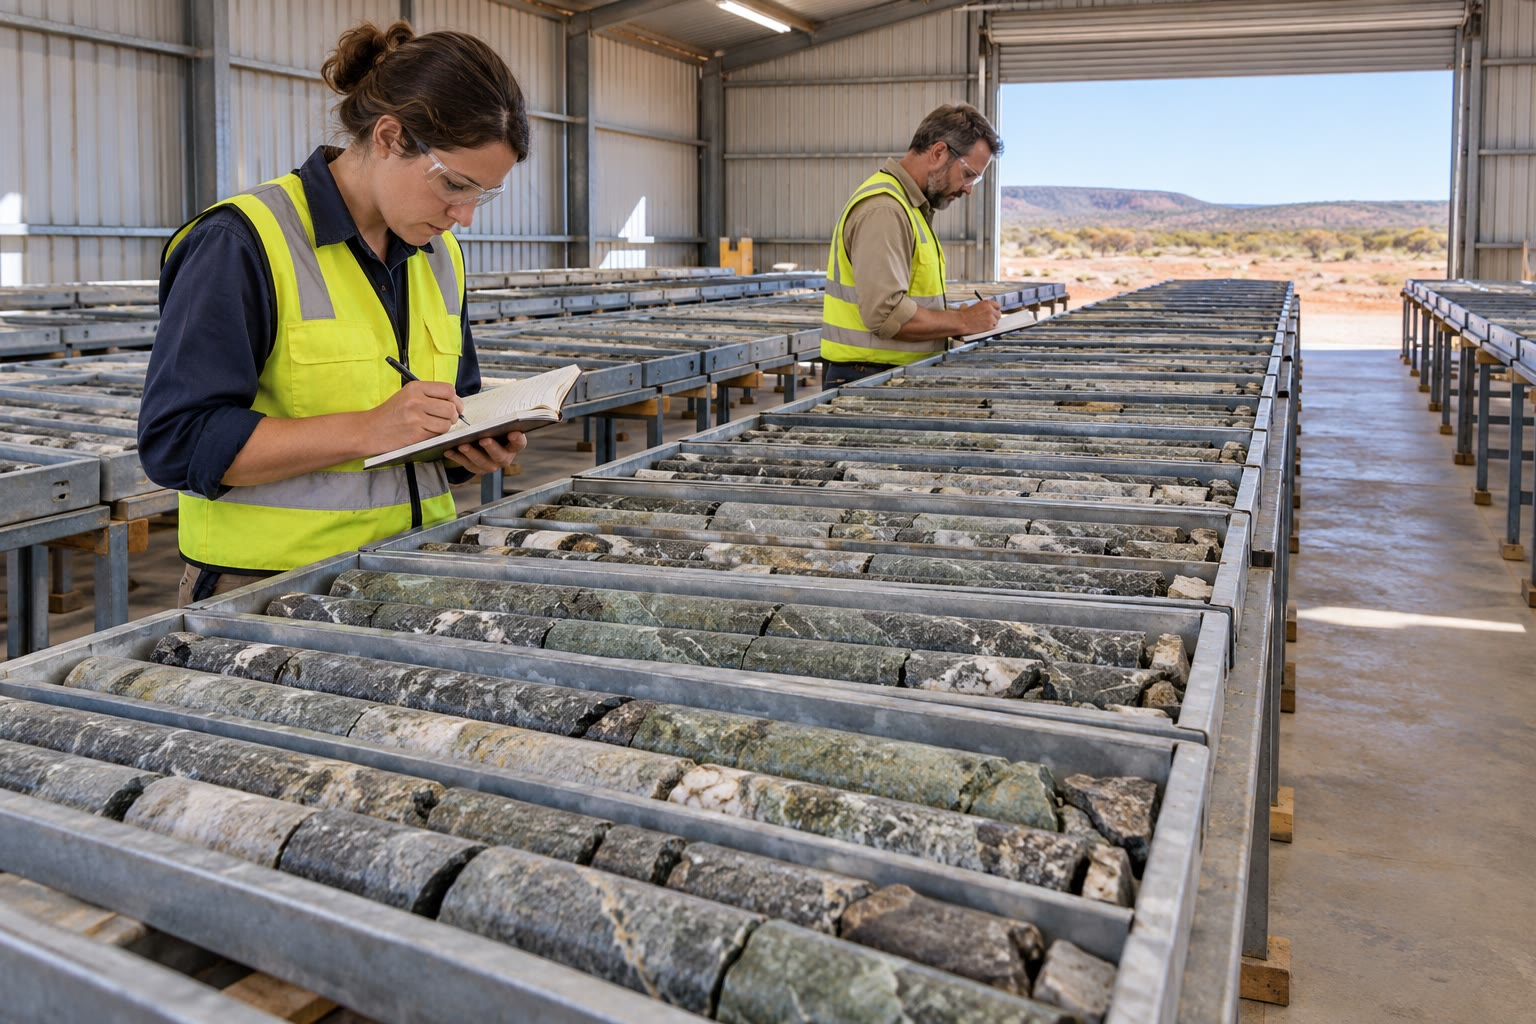
\includegraphics[width=0.56\linewidth]{images/book4/ai/b2-core-shed.jpg}
\par\smallskip{\small Una nave de testigos en un proyecto de exploración (ilustración generada por IA).}
\par\medskip\raggedright
En un proyecto de exploración, el testigo de cada sondeo se dispone en cajas metálicas en el orden
en que salió del terreno. Los geólogos recorren las cajas, tramo a tramo, y anotan qué
roca es, cómo está alterada, qué filones la cortan y en qué proporción, y qué sulfuros
contiene; marcan por dónde se cortará y muestreará el testigo. La descripción precede a los análisis y se
compara con ellos: una zona de alteración o un tipo de filón que lleva el metal se convierte en lo que hay que
seguir de un sondeo a otro, y a partir de la descripción los geólogos dibujan los cortes con los que se planifican los
sondeos siguientes.
\end{inthefield}

\section*{Ejercicios}\label{sec:b2:ore-deposits:exercises}

Datos de los ejercicios, salvo aviso contrario: corteza continental superior, cobre \qty{28}{ppm},
oro \qty{1.5}{ng/g}, cromo \qty{92}{ppm}; la población de pórfidos cupríferos de la
\cref{sec:b2:ore-deposits:grade-tonnage}, \omterm{def:b2:ore-deposits:grade}{tonelaje} (Mt) en $\log_{10}$ de media 2.373 y desviación
típica 0.654, \omterm{def:b2:ore-deposits:grade}{ley} (\%) en $\log_{10}$ de media $-0.364$ y desviación típica 0.199, correlación
$\rho = 0.100$. Redondéese a tres cifras significativas.
% ledger: rg03:ucc-trace, data:b4-porphyry-cu

\begin{exercise}[$\star$]\label{exo:b2:ore-deposits:1}
Hállese el \omterm{def:b2:ore-deposits:cf}{factor de concentración} respecto de la corteza superior de: (a) una mena de cobre al
\qty{0.5}{\percent}; (b) una mena de oro de \qty{6}{g/t}; (c) una cromitita con un \qty{90}{\percent}
de cromita, tomando la cromita como FeCr$_2$O$_4$ (masas atómicas Cr 52.00, Fe 55.85, O 16.00).
\end{exercise}

\begin{exercise}[$\star$]\label{exo:b2:ore-deposits:2}
Batu Hijau figura con \qty{914}{Mt} al \qty{0.53}{\percent} de Cu y \qty{0.40}{g/t} de Au por encima de una \omterm{def:b2:ore-deposits:grade}{ley de corte} del
\qty{0.3}{\percent}, y con \qty{1640}{Mt} al \qty{0.44}{\percent} de Cu y \qty{0.45}{g/t}
de Au para la \omterm{def:b2:ore-deposits:grade}{ley de corte} más baja disponible. (a) Hállense el cobre (Mt) y el oro (t) contenidos en cada
estimación. (b) ¿Qué \omterm{def:b2:ore-deposits:grade}{tonelaje} y qué cobre añaden los bloques adicionales de la segunda estimación, y con
qué \omterm{def:b2:ore-deposits:grade}{ley} media? (c) ¿Por qué son correctas ambas estimaciones?
\end{exercise}

\begin{exercise}[$\star$]\label{exo:b2:ore-deposits:3}
En la ley de Stokes, la velocidad de sedimentación de un grano de diámetro $d$ es proporcional a $(\rho_s -
\rho_w)\,d^2$. Tómense $\rho_w = 1.00$, cuarzo 2.65, oro 19.3, circón 4.7 (en
\unit{g.cm^{-3}}). (a) ¿Cuántas veces más deprisa sedimenta un grano de oro que un grano de cuarzo del
mismo tamaño? (b) ¿Cuál es la razón entre los diámetros de un grano de oro y uno de cuarzo que sedimentan a la
misma velocidad? (c) ¿Qué grano de cuarzo sedimenta como un grano de circón de \qty{0.1}{mm}?
\end{exercise}

\begin{exercise}[$\star$]\label{exo:b2:ore-deposits:4}
Una mena primaria de cobre tiene una \omterm{def:b2:ore-deposits:grade}{ley} del \qty{0.4}{\percent}. La meteorización lixivia todo su cobre en un
espesor de \qty{150}{m} y lo vuelve a depositar en una capa de \qty{50}{m} de espesor justo debajo, con la misma
densidad. (a) Hállese la \omterm{def:b2:ore-deposits:grade}{ley} de la capa. (b) Lo mismo si solo se vuelve a depositar el \qty{80}{\percent} del
cobre lixiviado. (c) ¿Qué espesor lixiviado daría un \qty{1.7}{\percent} si todo
el cobre se volviera a depositar?
\end{exercise}

\begin{exercise}[$\star\star$]\label{exo:b2:ore-deposits:5}
Un \omterm{def:b2:magma-emplacement:magma}{magma} contiene \qty{10}{ppb} de platino y \qty{200}{ppm} de níquel; tómense $D_{\mathrm{Pt}} =
10^4$ y $D_{\mathrm{Ni}} = 500$. (a) Con \eqref{eq:b2:ore-deposits:r-factor}, hállense los contenidos en
platino (ppm) y en níquel (\% en peso) del sulfuro para $R = 100$, \num{1000}, \num{10000}
y \num{100000}. (b) Hállense sus límites cuando $R \to \infty$. (c) Explíquese por qué una mena de níquel dice
poco sobre $R$, y una mena de platino mucho.
\end{exercise}

\begin{exercise}[$\star\star$]\label{exo:b2:ore-deposits:6}
Con \eqref{eq:b2:ore-deposits:product} para la población de pórfidos cupríferos: (a) hállense la media y la
desviación típica de $\log_{10} M$, y el cobre contenido mediano. (b) ¿Qué fracción de los yacimientos
contiene más de \qty{10}{Mt} de cobre? ¿Cuántos de los 422? (c) Repítase (b) sin tener en cuenta la correlación.
\end{exercise}

\begin{exercise}[$\star\star$]\label{exo:b2:ore-deposits:7}
Para el yacimiento ilustrativo de la figura ($T_0 = \qty{1000}{Mt}$, mediana del \qty{0.40}{\percent},
$s = 0.60$), úsese \eqref{eq:b2:ore-deposits:gt} para hallar el \omterm{def:b2:ore-deposits:grade}{tonelaje}, la \omterm{def:b2:ore-deposits:grade}{ley} media y el cobre contenido
por encima de \omterm{def:b2:ore-deposits:grade}{leyes de corte} del \qty{0.3}{\percent} y del \qty{0.6}{\percent}. Compruébese un punto en la figura.
\end{exercise}

\begin{exercise}[$\star\star$]\label{exo:b2:ore-deposits:8}
Un yacimiento de pórfido contiene \qty{5}{Mt} de cobre. Supóngase que su fluido magmático transportaba \qty{1000}{ppm}
de cobre, de las que la mitad se depositó en la mena, y que el \omterm{def:b2:magma-emplacement:magma}{magma} liberó el \qty{3.5}{\percent}
de su masa como fluido. (a) Hállense la masa de fluido y la de \omterm{def:b2:magma-emplacement:magma}{magma} necesarias. (b) Hállese el volumen del
\omterm{def:b2:magma-emplacement:magma}{magma}, de densidad \qty{2600}{kg.m^{-3}}. (c) Si el \omterm{def:b2:magma-emplacement:magma}{magma} contenía \qty{50}{ppm} de cobre, ¿qué fracción
de él acabó en la mena?
\end{exercise}

\begin{exercise}[$\star\star$]\label{exo:b2:ore-deposits:9}
Ocho sedimentos fluviales de fondo dan $\log_{10}$ Cu (ppm) de 1.30, 1.45, 1.38, 1.52, 1.41, 1.35,
1.48 y 1.40. (a) Hállense la media y la desviación típica (poblacional) de los logaritmos, la
mediana del fondo y el umbral media más dos desviaciones típicas, en ppm. (b) Un afluente
que drena \qty{4}{km^2} de terreno mineralizado lleva sedimento con \qty{400}{ppm}; se une a un río
que drena \qty{36}{km^2} con la mediana del fondo. Suponiendo que cada kilómetro cuadrado aporta la misma
masa de sedimento, ¿es anómalo el sedimento mezclado? (c) ¿Hasta qué superficie total de cuenca se mantiene la
anomalía por encima del umbral?
\end{exercise}

\begin{exercise}[$\star\star\star$]\label{exo:b2:ore-deposits:10}
(a) Demuéstrese que $e^{su}\varphi(u) = e^{s^2/2}\varphi(u - s)$. (b) Dedúzcase la media de una variable
lognormal, $e^{\mu + s^2/2}$. (c) Demuéstrese que la fracción del metal por encima de la \omterm{def:b2:ore-deposits:grade}{ley de corte},
$\Phi(z + s)$, siempre supera la fracción del \omterm{def:b2:ore-deposits:grade}{tonelaje}, $\Phi(z)$, e interprétese.
\end{exercise}

\begin{exercise}[$\star\star\star$]\label{exo:b2:ore-deposits:11}
(a) A partir de \eqref{eq:b2:ore-deposits:r-factor}, hállese el $R$ para el que $C_S$ alcanza una fracción $f$
de su techo $D\,C_L$. (b) Evalúese para $f = 0.5$ y $0.9$ con $D = 300$ (níquel) y $D =
10^4$ (platino). (c) Compárese con los intervalos de $R$ de las menas de níquel y cobre y de los niveles de EGP dados
en el texto.
\end{exercise}

\begin{exercise}[$\star\star\star$]\label{exo:b2:ore-deposits:12}
(a) Para una variable lognormal $M$ con $\ln M$ de desviación típica $s$, demuéstrese que los yacimientos por encima
del cuantil de orden $q$ contienen una fracción $\Phi\bigl(s - \Phi^{-1}(q)\bigr)$ del metal total.
(b) Evalúese para la población de pórfidos y $q = 0.9$. (c) Lo mismo para $q = 0.99$; compárese con
los cuatro yacimientos mayores, que contienen el \qty{26.6}{\percent} del cobre de la compilación.
\end{exercise}
% ledger: data:b4-porphyry-cu

\begin{problem}[{Problema de fin de semana --- Un prospecto de pórfido}]\label{pb:b2:ore-deposits:1}
Se ha perforado un prospecto de pórfido (inventado). Su sondeo de descubrimiento cortó ocho tramos, de arriba
abajo (longitud en metros, \omterm{def:b2:ore-deposits:grade}{ley} de cobre en tanto por ciento): 30 m al 0.12; 40 al 0.35; 50 al 0.62; 60
al 0.48; 40 al 0.27; 30 al 0.81; 50 al 0.41; 30 al 0.18. Un estudio geoestadístico de todos los sondeos
concluye que las \omterm{def:b2:ore-deposits:grade}{leyes} de los bloques son lognormales, con mediana del \qty{0.38}{\percent} y $s = 0.55$ para
$\ln g$. El cuerpo mineralizado se aproxima a un cilindro vertical de radio \qty{450}{m} y altura
\qty{700}{m}, de densidad \qty{2.7}{t.m^{-3}}. Úsense los datos de los ejercicios y redondéese a tres
cifras significativas (las probabilidades a cuatro).

\noindent\textbf{Parte I --- El sondeo de descubrimiento.}
\begin{enumerate}
  \item Hállense la longitud muestreada del sondeo y su \omterm{def:b2:ore-deposits:grade}{ley} media ponderada por la longitud.
  \item Hállese la media aritmética de las ocho \omterm{def:b2:ore-deposits:grade}{leyes}. ¿Por qué es la media ponderada la correcta?
  \item ¿Qué fracción de la longitud supera el \qty{0.3}{\percent}, y con qué \omterm{def:b2:ore-deposits:grade}{ley} media?
  \item Hállese el \omterm{def:b2:ore-deposits:cf}{factor de concentración} de la \omterm{def:b2:ore-deposits:grade}{ley} media ponderada respecto de la corteza superior.
  \item Lo mismo para el tramo más rico.
  \item Hállese la \omterm{def:b2:ore-deposits:grade}{ley} media de todos los bloques del yacimiento. ¿Es representativo el sondeo de descubrimiento?
\end{enumerate}

\noindent\textbf{Parte II --- Tonelaje por encima de la ley de corte.}
\begin{enumerate}[resume]
  \item Hállense el volumen y el \omterm{def:b2:ore-deposits:grade}{tonelaje} $T_0$ del cuerpo; consérvese $T_0 = \qty{1200}{Mt}$.
  \item Para una \omterm{def:b2:ore-deposits:grade}{ley de corte} del \qty{0.3}{\percent}, hállense $z$ y la fracción de los bloques que la superan.
  \item Hállese el \omterm{def:b2:ore-deposits:grade}{tonelaje} por encima de \omterm{def:b2:ore-deposits:grade}{leyes de corte} del 0.2, del 0.3 y del \qty{0.5}{\percent}.
  \item Hállese la \omterm{def:b2:ore-deposits:grade}{ley} media por encima de la \omterm{def:b2:ore-deposits:grade}{ley de corte} del \qty{0.3}{\percent}.
  \item Lo mismo por encima del 0.2 y del \qty{0.5}{\percent}.
  \item Al subir la \omterm{def:b2:ore-deposits:grade}{ley de corte} del 0.3 al \qty{0.5}{\percent}, ¿por qué factores cambian el \omterm{def:b2:ore-deposits:grade}{tonelaje} y la
        \omterm{def:b2:ore-deposits:grade}{ley} media?
  \item ¿Con qué \omterm{def:b2:ore-deposits:grade}{ley de corte} se conserva la mitad del \omterm{def:b2:ore-deposits:grade}{tonelaje}, y cuál es su \omterm{def:b2:ore-deposits:grade}{ley} media?
\end{enumerate}

\noindent\textbf{Parte III --- El prospecto entre los pórfidos del mundo.}
\begin{enumerate}[resume]
  \item Hállese el cobre contenido en todo el cuerpo, con su \omterm{def:b2:ore-deposits:grade}{ley} media.
  \item Hállese la puntuación tipificada de su \omterm{def:b2:ore-deposits:grade}{tonelaje} en la población mundial, y su percentil.
  \item Lo mismo para su \omterm{def:b2:ore-deposits:grade}{ley} media.
  \item Hállese la desviación típica de $\log_{10} M$ con la correlación y sin ella.
  \item Hállese el percentil de su cobre contenido.
  \item ¿Cuántos de los 422 yacimientos cabría esperar que contengan más cobre?
\end{enumerate}

\noindent\textbf{Parte IV --- El cobre por encima de la ley de corte.}
\begin{enumerate}[resume]
  \item Hállese el cobre contenido por encima de la \omterm{def:b2:ore-deposits:grade}{ley de corte} del \qty{0.2}{\percent}.
  \item Lo mismo por encima del \qty{0.5}{\percent}.
  \item ¿Qué fracción del cobre se encuentra por encima del \qty{0.3}{\percent}, y qué fracción del
        \omterm{def:b2:ore-deposits:grade}{tonelaje}?
  \item Explíquese por qué bajar la \omterm{def:b2:ore-deposits:grade}{ley de corte} por debajo del \qty{0.3}{\percent} añade mucha roca y poco
        cobre, usando las respuestas a las preguntas 9 y 20.
  \item En resumen: ¿cuánto cobre contiene el prospecto por encima de la \omterm{def:b2:ore-deposits:grade}{ley de corte} del \qty{0.3}{\percent}?
\end{enumerate}
\end{problem}
